\tasknumber{2018}{9} Построить график: $y=\dfrac{|x^2-5x+6|}{x-2}$\\
\begin{center}
Разложим числитель на множители по теореме Безу:
$x^2-5x+6=(x-2)(x-3) \hm\Rightarrow$\\
При $ x \in (-\infty; 2)\cup (3; +\infty): (x-2)(x-3)\geqslant 0,$ при $ x \in (2;3]: (x-2)(x-3)<0 $\\
1)При $x \in (-\infty; 2)\cup (3; +\infty): y=\dfrac{(x-2)(x-3)}{x-2} \Leftrightarrow \left\{
\begin{array}{l}
y=x-3,\\
x\neq2.
\end{array} 
\right. $\\
2)При $x \in (2;3], y=-\dfrac{(x-2)(x-3)}{x-2}\Leftrightarrow \left\{
\begin{array}{l}
y=3-x,\\
x\neq2.
\end{array} \right.$\\
 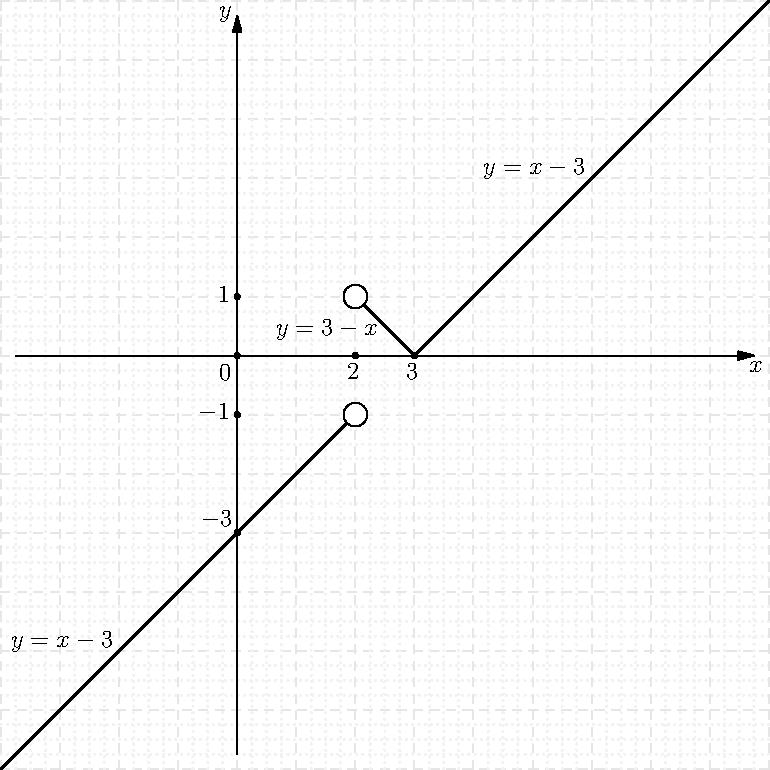
\includegraphics[scale =1]{graphic.pdf}
\end{center}